\documentclass[UTF8]{ctexart}
\usepackage[left=2cm,right=2cm,top=1.5cm,bottom=1.5cm]{geometry}
\usepackage{listings}
\usepackage{xcolor}
\usepackage{fontspec}
\usepackage{amsmath}
\usepackage{tikz}
\usetikzlibrary{calc}
\usepackage[thmmarks,amsmath]{ntheorem}
\setmonofont{Consolas}

\begin{document}
	\title{算法基础第二次作业}
	\author{肖桐 PB18000037}
	\date{2020 年 10 月 13 日}
	\maketitle

	\newtheorem*{solution}{解}

	\begin{solution}\textnormal{\textbf{1.}}
		若题目要求排序结果为升序排列, 则对应的堆排序就要建立最大堆.\newline
		(1). 此时若初始数组$A$为升序排列, 实际上对建堆过程没有特殊贡献, 建堆复杂度仍然为$O(n)$. 接着进行堆排序所需的复杂度为$O(n\lg n)$.\newline
		因此总的复杂度为$O(n\lg n)$.\newline
		(2). 若初始数组$A$为降序排列, 则此时建堆过程复杂度为$O(1)$, 即相当于最大堆已经建好. 接下来进行堆排序的复杂度仍然为$O(n\lg n)$.\newline
		因此总的复杂度仍然为$O(n\lg n)$.\newline
		若题目要求排序结果为降序排列, 对应的堆排序需要建立最小堆. 则当$A$为升序排列时建堆时间为$O(1)$, $A$降序时建堆时间为$O(n)$, 但总的排序复杂度都为$O(n\lg n)$.
	\end{solution}
	\begin{solution}\textnormal{\textbf{2.}}
		(a). 因为$0 \leq \alpha \leq \dfrac{1}{2}$, 因此$\alpha < 1 - \alpha$. 故每次划分比例为$\alpha$的部分会最早到达叶节点.
		每次划分比例为$1 - \alpha$的部分会最晚到达叶节点\newline
		假设叶节点最小深度为$h_1$, 因为叶节点节点个数为$1$, 则令$n\alpha^{h_1} = 1$, 两边取对数即可解得:$h_1 = -\dfrac{\lg n}{\lg\alpha}$\newline
		设叶节点最大深度为$h_2$, 则同理可令$n(1 - \alpha)^{h_2} = 1$, 两边取对数可解得:$h_2 = -\dfrac{\lg n}{\lg(1 - \alpha)}$\newline
		(b). 假设该随机数组有$n$个元素, 每个元素作为主元的概率都相等, 都为$\dfrac{1}{n}$.\newline
		假设这$n$个元素升序排序如下:\newline\newline
		\rm{
		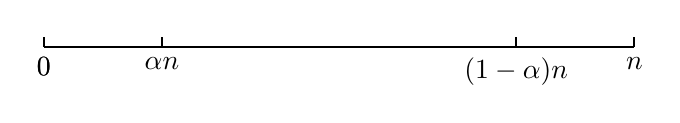
\begin{tikzpicture}[>=stealth,scale=1,line width=0.8pt]
			%\useasboundingbox[draw](-1,-1) rectangle(9,6);
			% % % % % % % % % % % % % % %
			\pgfmathsetmacro{\ticker}{0.125} %ticker的长度 
			%画一个矩形
			\coordinate (A) at (0,0);
			%\coordinate (B) at (0,5);
			%\coordinate (C) at (7.5,5);
			\coordinate (D) at (7.5,0);
			%\draw(A)--(B)--(C)--(D)--cycle;
			\draw(A)--(D);
			%标注xy
			%\coordinate [label=left:$\frac{\theta}{\theta _{0}}$](E) at ($(B)+(-0.4,-0.2)$);
			%\coordinate [label=below:$Bi \cdot Fo $](F) at ($(D)+(-0.2,-0.4)$);
			%绘制ticker
			%\foreach \i/\texti  in {1,2,3,4,5} {
			%\draw (1.5*\i,0) --(1.5*\i,\ticker) node[label=below:\texti]{};
			%}
			\draw (0, 0) -- (0, \ticker) node[label=below: $0$]{};
			\draw (1.5, 0) -- (1.5, \ticker) node[label=below: $\alpha n$]{};\draw (0, 0) -- (0, \ticker) node[label=below: $0$]{};
			\draw (6, 0) -- (6, \ticker) node[label=below: $(1 - \alpha)n$]{};
			\draw (7.5, 0) -- (7.5, \ticker) node[label=below: $n$]{};
			%\foreach \j/\textj  in {0.2,0.4,0.6,0.8,1.0} {
			%\draw (0,5*\j) --(\ticker,5*\j) node[label=left:\textj]{};
			%}
			%绘制miniticker
			%\foreach \i  in {0.5,1.5,...,4.5} {
			%\draw (1.5*\i,0) --(1.5*\i,0.8*\ticker);
			%}
			%\foreach \j  in {0.1,0.3,...,0.9} {
			%\draw (0,5*\j) --(0.8*\ticker,5*\j);
			%}
		\end{tikzpicture}
		}\newline
		易知选取$\alpha n$点或$(1 - \alpha)n$点作为主元进行切分则满足切分比为$(1 - \alpha):\alpha$,
		若要比$(1 - \alpha):\alpha$更平均, 则选取的主元应该在$\alpha n$和$(1 - \alpha)n$之间, 共有$(1 - 2\alpha)n$个点.\newline
		故比$(1 - \alpha):\alpha$更平均的概率为:$(1 - 2\alpha)n \cdot \dfrac{1}{n} = 1 - 2\alpha$
	\end{solution}
\end{document}